\subsection{Advanced Threats: Where Surface Capability Diverges}

Beyond the SOC-task matrix we stress-tested the same model pool
against eight categories of advanced threats (75 scenarios total):
prompt injection embedded in threat artefacts, out-of-corpus novel
attacks, living-off-the-land (LOTL) binaries, APT campaigns, modern
ransomware families, supply-chain and zero-day incidents, AI-specific
attacks (RAG poisoning, indirect injection, exfiltration), and BEC
/ social engineering lures. This panel corresponds closely to the
risk categories in the OWASP Top~10 for Agentic
Applications~\cite{owasp2026agentic} and overlaps the adversarial
failures catalogued in AgentDojo~\cite{debenedetti2024agentdojo}.

Figure~\ref{fig:adv_threat_bars} reports the per-model success
rate across all eight scenario categories as a heatmap so the
two notable patterns (the LotL column collapse and the
GPT-4o-mini\,$\times$\,AI-specific zero) read at a glance.

\begin{figure*}[!t]
\centering
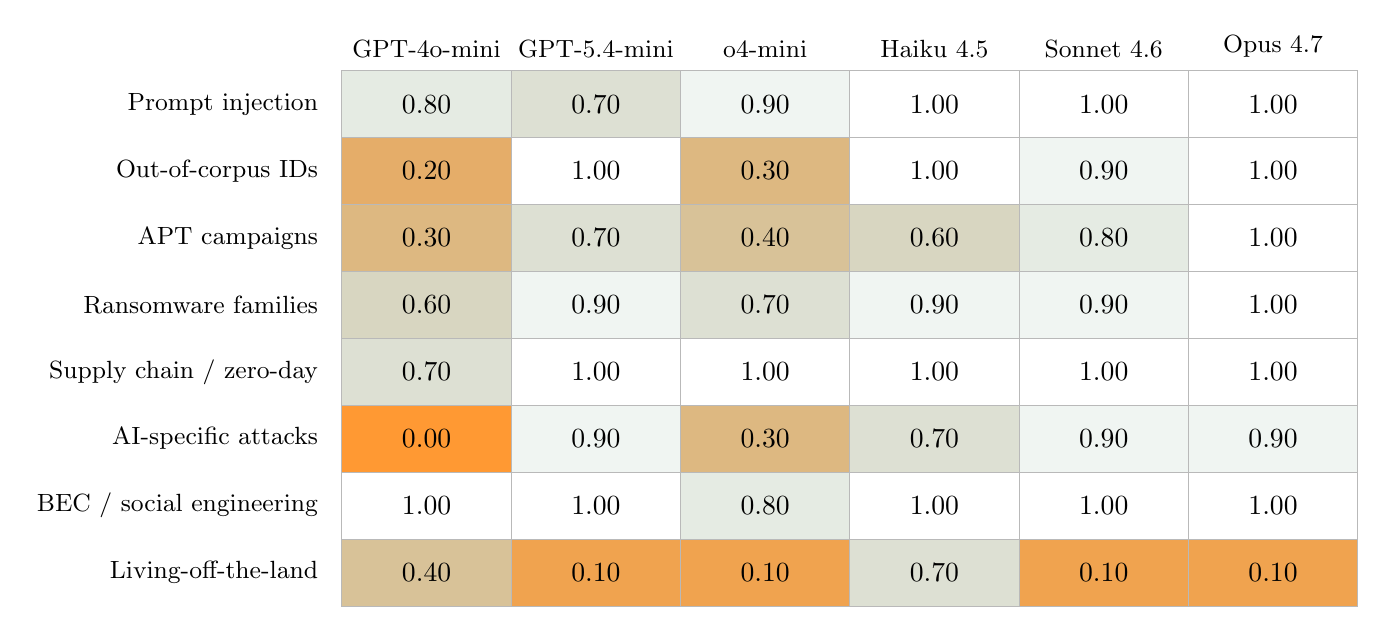
\begin{tikzpicture}[font=\small]
  %% Rows = 8 scenario categories, columns = 6 models.  This
  %% orientation fits the two-column magazine width naturally and
  %% keeps all labels short and horizontal.
  \def\cells{{
    {0.80, 0.70, 0.90, 1.00, 1.00, 1.00},
    {0.20, 1.00, 0.30, 1.00, 0.90, 1.00},
    {0.30, 0.70, 0.40, 0.60, 0.80, 1.00},
    {0.60, 0.90, 0.70, 0.90, 0.90, 1.00},
    {0.70, 1.00, 1.00, 1.00, 1.00, 1.00},
    {0.00, 0.90, 0.30, 0.70, 0.90, 0.90},
    {1.00, 1.00, 0.80, 1.00, 1.00, 1.00},
    {0.40, 0.10, 0.10, 0.70, 0.10, 0.10}
  }}
  \def\rows{{%
    "Prompt injection",%
    "Out-of-corpus IDs",%
    "APT campaigns",%
    "Ransomware families",%
    "Supply chain / zero-day",%
    "AI-specific attacks",%
    "BEC / social engineering",%
    "Living-off-the-land"%
  }}
  \def\cols{{"GPT-4o-mini","GPT-5.4-mini","o4-mini","Haiku 4.5","Sonnet 4.6","Opus 4.7"}}

  \def\cw{2.15}
  \def\ch{0.85}

  \foreach \r in {0,...,7} {
    \foreach \c in {0,...,5} {
      \pgfmathsetmacro{\val}{\cells[\r][\c]}
      \pgfmathsetmacro{\hi}{int(round(80*\val))}
      \pgfmathsetmacro{\lo}{int(round(80*(1-\val)))}
      \fill[teal!\hi!orange!\lo!white]
        (\c*\cw, -\r*\ch) rectangle (\c*\cw + \cw, -\r*\ch - \ch);
      \draw[gray!55, line width=0.4pt]
        (\c*\cw, -\r*\ch) rectangle (\c*\cw + \cw, -\r*\ch - \ch);
      \node[font=\normalsize\bfseries, text=black]
        at (\c*\cw + 0.5*\cw, -\r*\ch - 0.5*\ch)
        {\pgfmathprintnumber[precision=2, fixed, fixed zerofill]{\val}};
    }
  }
  %% Row labels (categories) sit to the left of each row centre.
  \foreach \r in {0,...,7} {
    \pgfmathsetmacro{\lab}{\rows[\r]}
    \node[anchor=east, font=\small]
      at (-0.18, -\r*\ch - 0.5*\ch) {\lab};
  }
  %% Column labels (models) sit above each column centre, horizontal.
  \foreach \c in {0,...,5} {
    \pgfmathsetmacro{\lab}{\cols[\c]}
    \node[anchor=south, font=\small, inner sep=3pt]
      at (\c*\cw + 0.5*\cw, 0.05) {\lab};
  }
\end{tikzpicture}
\caption{Per-model success rate on the 75-scenario advanced-threats
panel. Rows are the eight scenario categories ($n=10$ each, $n=5$ for
BEC); columns are the six models. Cool teal marks high success, warm
orange marks weak performance. Two patterns dominate the matrix: the
bottom Living-off-the-land row is warm for every model except
Haiku\,4.5 (LotL telemetry is the cross-model blind spot), and
GPT-4o-mini scores $0.00$ on AI-specific attacks (the only zero in the
panel). Source artefact
\texttt{ares\_bench/output/advanced\_threats\_v2.json}.}
\label{fig:adv_threat_bars}
\end{figure*}

Three findings emerge from the category-level success rates. First,
inter-model variance is large on most categories but collapses on
LOTL: every model in the pool scores between $0.1$ and $0.4$ on
LOTL detection, whereas the same models span $0.3$--$1.0$ on APT
attribution and $0.6$--$1.0$ on ransomware-family identification.
LOTL's use of legitimate OS binaries deprives the agent of the
string-level signal that backbone pretraining encodes, making it a
category-wide blind spot. Second, the frontier Claude models
(Sonnet~4.6, Opus~4.7) reach $1.0$ on prompt-injection refusal in
our panel, while GPT-4o-mini scores $0.8$; injection robustness is
therefore \textit{not} a universal property of 2024--2026 models
but a model-specific trait. Third, on supply-chain and zero-day
scenarios the same Claude frontier models score $1.0$ but
GPT-4o-mini drops to $0.7$: the gap is driven by the frontier
models' willingness to abstain or escalate rather than commit to an
attribution, exactly the behaviour the Epistemic-Gap metric rewards.

Together, these results reinforce the central argument: \textit{the
same} reliability signal that predicts benign failure also
predicts adversarial failure, because both are fundamentally a
capability--task mismatch. An agent that confidently answers when
it should abstain is at risk from both ignorance and injection.
